\section{Experimental results}
\label{results}
\subsection{Datasets and evaluation protocol}
\label{subsec:datasets}
We use public datasets and corresponding evaluation protocol proposed by each dataset author. 

\textbf{HMDB51} \cite{kuehne2011} includes a large collection of human activities categorized on 51 classes. It collects 6766 videos from different media resources \ie digitized movies, public databases and user generated web video data. We adopt the evaluation protocol proposed by the authors evaluating performance as mean accuracy under three fixed train/test splits.

\textbf{Hollywood2} \cite{marszalek2009} contains a wide number of videos retrieved from 69 different Hollywood movies. It is divided in 12 categories including short actions such as Kiss, Answer Phone and Stand Up. This dataset presents a lot of challenges for action recognition approches due to the several change of camera view point and the unchoreographed action execution. We follow the initial evaluation protocol where videos are splited in a training set of 823 videos a testing set of 884 videos. To measure recognition performance, we compute the mean average precision (mAP) over all dataset 
classes.

\textbf{Olympic Sports} \cite{niebles2010} consists of 783 YouTube videos of sports related human movements. The recognition performance is measured 
by the mAP computed over 134 testing sequences. Videos are annotated using Amazon Mechanical Turk as 16 different olympic sports \eg pole vault, springboard and hammer throw.

\textbf{UCF50} \cite{reddy2013} includes 6618 videos of 50 different human actions. This data set is an extension of the YouTube Action dataset (UCF11) which has 11 action categories. This dataset presents several recognition challenges due to large variations in camera motion, cluttered background, viewpoint etc. Action categories are grouped into 25 sets, where each set consists of more than 4 action clips. Recognition performance is measured by applying a leave-one-group-out cross-validation and report the average accuracy over all group splits. 

\subsection{Implementation details}

\textbf{Visual descriptors}. Foreground descriptors \ie Trajectory Shape, HOG, HOF, and MBH are computed using a modified implementation of the method presented by \cite{wang2013}. Instead of compensating camera motion using a Homography, we compute a Fundamental Matrix to robustly find inliers matches for warping consecutive frames. To describe the visual contextual appearance, we extract SIFT \cite{lowe2004} on non-foreground regions (See previous section). Moreover, we fit a refined Fundamental Matrix in order to weakly model the camera motion. It is computed using RANSAC from inliers points resulting on the camera compensation step. \\\\
\textbf{Codebook generation}. We adopt two different approaches: (a) \textit{k}-means, where we learn a partitioning space for each descriptor type and (b) a Gaussian Mixture Model (GMM), where we capture the probability of each descriptor separately. Because of there are a large amount of features we have to sub-sample the visual world. We have noticed the impact of this sub-sampling on recognition performance as observed in Figure \ref{fig:feature_sampling}. We argue that sampling a small amount of features results on poor partitioning of the visual space. Motivated by this analysis, we commonly sample the 5\% of each features for our codebook generation approaches in all datasets. Moreover, we sub-sample features using a spatial clustering of feature points followed by a 1-Nearest Neighbor assignment. \\\\
\textbf{Feature encoding}. We follow the traditional histogram quantization (VQ) as one of our encoding strategies. Another type of encoding are the recently well-accepted Fisher Vectors (FV) \cite{perronnin2010}. For computing FV we have used the same implementation as provided in \cite{perronnin2010}. \\\\
\textbf{Normalization}. To make our representations robust to the number of extracted local descriptors, we normalize the final feature vector using one or a combination of the following techniques: (a) \textit{l2} normalization (L2) \cite{perronnin2010}, (b) power normalization (PW) \cite{perronnin2010} and (c) intra-normalization (IN) \cite{xwang2013}. \\\\
\textbf{Framework representation}. We adopt two majors frameworks for action recognition. One of them is following the Bag of words paradigm. We use \textit{k}-means for computing visual codebooks. Then, we encode features using the mentioned VQ strategy. Ultimately, we learn a non-linear SVM with $\chi^2$ kernel (MCSVM), combining our features using a multichannel approach as in \cite{zhang2007}:
\begin{equation}
K(x_i,x_j)= \exp(-\sum_c {\frac{1}{2\Omega_c} D_c(x_i,x_j)}),
\label{eq:multichannel}
\end{equation}
where $D_c(x_i,x_j)$ is the $\chi^2$ distance for channel $c$, and $\Omega_c$ is the average channel distance (see Table \ref{tab:frameworks}). Moreover, we implement a more robust framework (Fisher vectors) learning a codebook using a GMM. Consequently, we encode the feature vectors using \cite{perronnin2010}. In this case, we apply three normalization strategies, L2, PW and IN as proposed in \cite{xwang2013}. Finally, normalized channels are concatenated and action models are learned within a linear SVM.

%%%%%%%%%%%%%%%%% Figure: Effect of sampling %%%%%%%%%%%%%%%%%%%
\begin{figure*}[t!]
\begin{center}
%\fbox{\rule{0pt}{1.2in} \rule{0.9\linewidth}{0pt}}
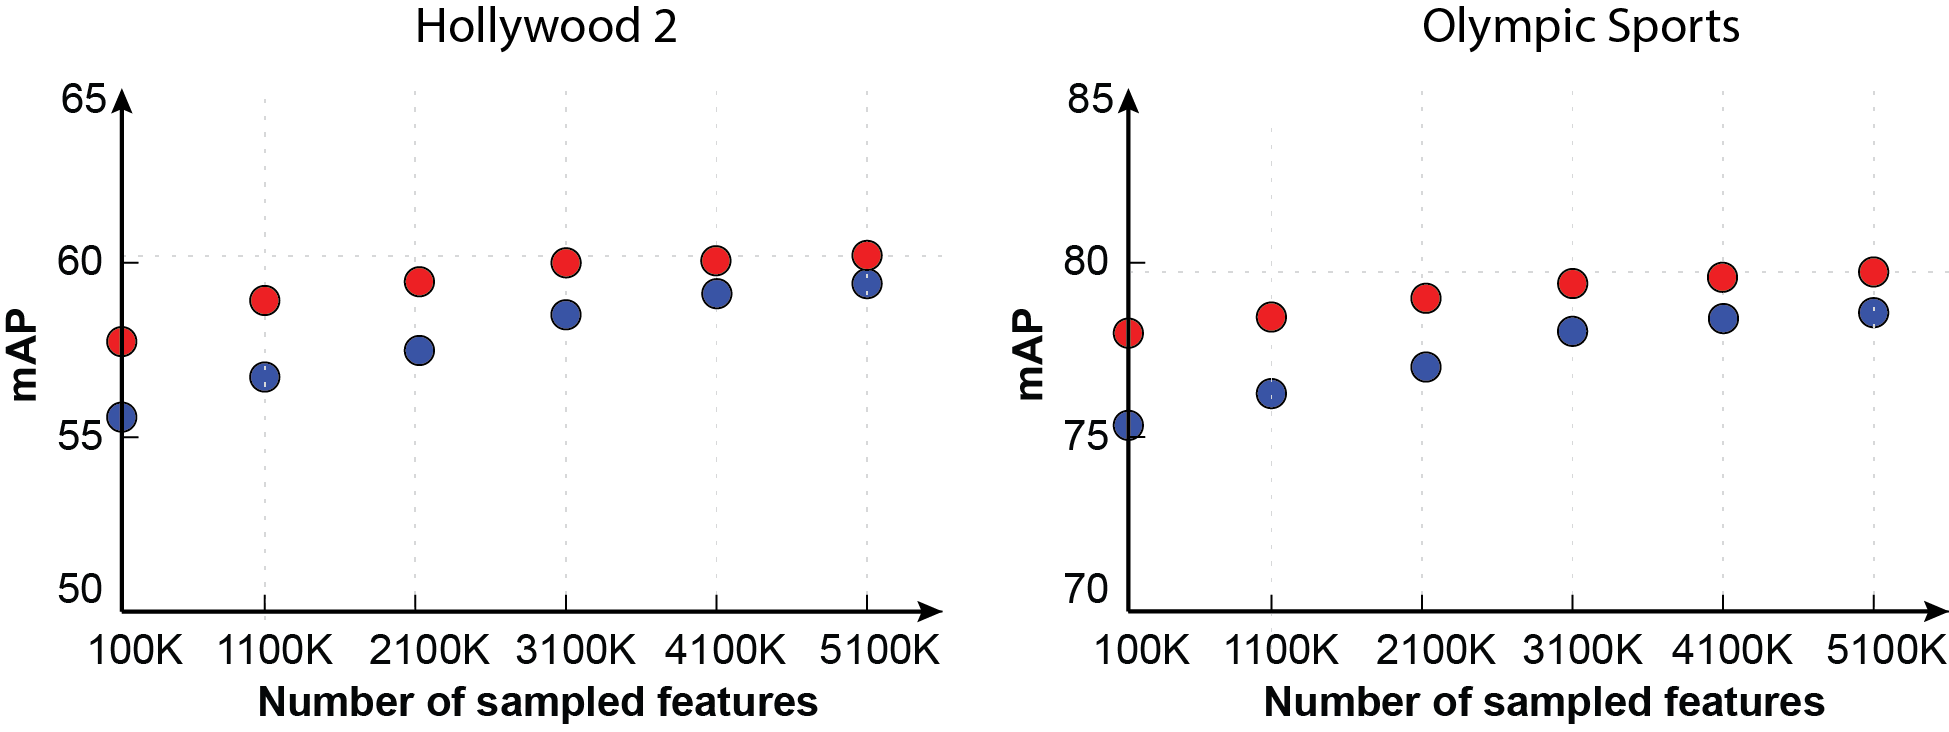
\includegraphics[width=0.98\linewidth]{fig/sampling.png}
\end{center}
\caption{Effect of feature sub-sampling when generating codebook.}
\label{fig:feature_sampling}
\end{figure*}
%%%%%%%%%%%%%%%%%%%%%%%%%%%%%%%%%%%%%%%%%%%%%%%%%%%%%%%%%%%%%%%%

%%%%%%%%%%%%%%% Table: Frameworks comparison %%%%%%%%%%%%%%%%%%%
\begin{table*}[h!]
\caption{Comparison of adopted frameworks for action recognition.}
\begin{center}
{
\begin{tabular}{ l| c c c c c }
\hline
Representation $\downarrow$ & Codebook & Encoding & Normalization & Classifier \\
\hline
Bag of words & \textit{k}-means & VQ & L2 & MCSVM \\
Fisher vectors & GMM & Fisher vectors & L2+PW+IN & LSVM \\
\hline
\end{tabular}
}
\end{center}
\label{tab:frameworks}
\end{table*}
%%%%%%%%%%%%%%%%%%%%%%%%%%%%%%%%%%%%%%%%%%%%%%%%%%%%%%%%%%%%%%%%

\subsection{Impact of surrounding features}
We conduct further experiments to measure the contribution of our context features. We compute and compare per-feature performance for the datasets described in Section \ref{subsec:datasets}. We define as baseline a representation that only includes foreground features to describe video sequences \cite{wang2013}. Table \ref{tab:features} summarize conducted experiments. Moreover, we investigate the effect of the representation used \ie Bag of words or Fisher vectors on the overall performance. \\\\
\textbf{Representation}. As suggested in recent works \cite{perronnin2010, wang2013, xwang2013} Fisher vectors representation provides a boost in performance compared to the traditional Bag of words. Our experiments shows that this improvements in performance are also included in our contextual features descriptors. However, we note that Fisher vectors representation is less important with our CamMotion descriptor. Consequently, Fisher vectors are used for our following analysis.\\\\
\textbf{Foreground-background}. As described in Section \ref{scene}, we perform a weak separation of background and foreground feature points. We measure the effect on performance of this separation for our contextual features. We note that this type of weak segmentation provides a significant boost in performance, as observed in Table \ref{tab:segmentation}. When feature points are localized on the background SIFT features capture useful information to encode the scene. Our CamMotion descriptor exhibit a poor performance when the fundamental matrix is computed with all matches points on the video. In that case fundamental matrix includes a large amount of outliers that correspond to matches from foreground regions. This problem is alleviated computing the global descriptor on the background feature points. \\\\
\textbf{Context appearance}. While by itself SIFT achieves a discrete performance, it produces notable improvements when combined with foreground descriptors. Table \ref{tab:features} reports obtained results on four benchmark datasets. Interestingly, we note that SIFT description produce better results in Olympic Sports and UCF50. This can be attributed to type of activities depicted on these datasets, which almost contains sport related activities.\\\\
\textbf{Camera motion} descriptor allows to add important cues for recognition in some datasets. While it provides a less improvement compared to our context appearance features, also shows a significant improvement when used on user-generated datasets. For example, in Olympic Sports using this low level descriptor, we boost the performance on ~2.2\%. Moreover, we evidence a consistent small contribution over all datasets.

%%%%%%%%%%%%% Table: Effect of selected points %%%%%%%%%%%%%
\begin{table*}
\caption{Effect of compute contextual features on background points.}
\begin{center}
{
\begin{tabular}{|c|c c|c c c c|}
\hline
& \multicolumn{2}{|c|}{Feature points} & \multicolumn{4}{|c|}{Datasets} \\
Feature $\downarrow$ & Foreground & Background & HMDB51 & Hollywood2 & Olympics & UCF50 \\
\hline
SIFT & \checkmark & & 19.5\% & 22.1\% & 33.5\% & 44.7\% \\
SIFT & & \checkmark & \textbf{20.1\%} & \textbf{28.5\%} & \textbf{39.6\%} & \textbf{49.8\%} \\
SIFT & \checkmark & \checkmark & 19.8\% & 24.3\% & 34.4\% & 45.9\% \\
\hline
CamMotion & \checkmark & & 9.7\% & 14.9\% & 19.5\% & 13.7\% \\
CamMotion & & \checkmark & \textbf{14.1\%} & \textbf{22.1\%} & \textbf{27.2\%} & \textbf{19.5\%} \\
CamMotion & \checkmark & \checkmark & 12.9\% & 18.7\% & 21.8\% & 17.2\% \\
\hline
\end{tabular}
}
\end{center}
\label{tab:segmentation}
\end{table*}
%%%%%%%%%%%%%%%%%%%%%%%%%%%%%%%%%%%%%%%%%%%%%%%%%%%%%%%%%%%%

%%%%%%%%%%%%%% Table: Feature analysis %%%%%%%%%%%%%%%%%%%%%
\begin{table*}
\caption{Impact of our contextual features on recognition performance.}
\begin{center}
{
\def\arraystretch{1.11}
\setlength{\tabcolsep}{3.66pt}
\begin{tabular}{ |c c c|c c c c| }
\hline
\multicolumn{3}{|c|}{Features} & \multicolumn{4}{|c|}{Datasets} \\
Foreground & SIFT & CamMotion & HMDB51 & Hollywood2 & Olympics & UCF50 \\
\hline
\multicolumn{7}{|c|}{Framework: Bag of words} \\
\hline
\checkmark & & & 51.2\% & 60.1\% & 79.8\% & 85.9\% \\
& \checkmark & & 19.5\% & 28.7\% & 36.4\% & 45.7\% \\
& & \checkmark & 13.5\% & 21.8\% & 26.9\% & 19.3\% \\
\checkmark & \checkmark & & 53.8\% & 60.9\% & 81.1\% & 87.2\% \\
\checkmark &  & \checkmark & 50.9\% & 60.4\% & 80.6\% & 86.8\% \\
& \checkmark & \checkmark & 20.7\% & 36.2\% & 43.7\% & 50.3\% \\
\checkmark & \checkmark & \checkmark & 51.7\% & 61.6\% & 81.7\% & 87.6\% \\
\hline
\multicolumn{7}{|c|}{Framework: Fisher vectors} \\
\hline
\checkmark & & & 56.5\% & 62.4\% & 90.4\% & 90.9\% \\
& \checkmark & & 20.1\% & 28.5\% & 39.6\% & 49.8\% \\
& & \checkmark & 14.1\% & 22.1\% & 27.2\% & 19.5\% \\
\checkmark & \checkmark & & \textbf{59.2\%} & \textbf{63.5\%} & \textbf{91.6\%} & \textbf{93.3\%} \\
\checkmark &  & \checkmark & 55.9\% & 62.9\% & 91.3\% & 93.1\% \\
& \checkmark & \checkmark & 22.3\% & 36.5\% & 46.5\% & 54.3\% \\
\checkmark & \checkmark & \checkmark & \textbf{57.9\%} & \textbf{64.1\%} & \textbf{92.5\%} & \textbf{93.8\%} \\
\hline
\end{tabular}
}
\end{center}
\label{tab:features}
\end{table*}
%%%%%%%%%%%%%%%%%%%%%%%%%%%%%%%%%%%%%%%%%%%%%%%%%%%%%%%%%%%%%


\subsection{Comparison with the state of the art}
We compare our method with recent works targeting the same application scenario and 
similar representations \ie works that uses dense trajectory points to represent video sequences \cite{wang2013, jiang2012, jain2013}. We also present results for our own implementation of \cite{wang2013}, which correspond to our baseline (Foreground). It is important to enhance that we achieve a slightly lower performance in our i mplementation of \cite{wang2013}. Experimental results show strong evidence of the contribution of our contextual features. We achieve state-of-the-art in all evaluated datasets, except in Hollywood 2 (see Table \ref{tab:stateofart}. We argue that our approach not include Human Detection (HD) for computing the Improved Trajectories and we expect further improvements if this strategy is included.  


%%%%%%%%%%%%%% Table: State-of-the-art %%%%%%%%%%%%%%%%%%%%%%
\begin{table*}
\caption{Comparison with the state-of-the-art on HMDB51, Hollywood2, Olympic Sports and UCF50 datasets.}
\begin{center}
{
\begin{tabular}{ |l| c c c c| }
\hline
Approach $\downarrow$ & HMDB51 & Hollywood2 & Olympics & UCF50 \\
\hline
Jiang \etal \cite{jiang2012} & 40.7\% & 59.5\% & 80.6 & - \\
Jain \etal \cite{jain2013} & 52.1\% & 62.5\% & 83.2 & - \\
Wang \etal \cite{wang2013} non-HD & 55.9\% & 63.0\% & 90.2\% & 90.5\% \\
Wang \etal \cite{wang2013} HD & 57.2\% & \textbf{64.3\%} & 91.1\% & 91.2\% \\
\hline
\multicolumn{5}{|c|}{\textit{Our methods with FV}} \\
\hline
Baseline (Foreground) & 56.5\% & 62.4\% & 90.4\% & 90.9\% \\
Foreground + SIFT & \textbf{59.2\%} & 63.5\% & \textbf{91.6\%} & \textbf{93.3\%} \\
Foreground + SIFT + CamMotion  & \textbf{57.9\%} & \textbf{64.1\%} & \textbf{92.5\%} & \textbf{93.8\%} \\
\hline
\end{tabular}
}
\end{center}
\label{tab:stateofart}
\end{table*}
%%%%%%%%%%%%%%%%%%%%%%%%%%%%%%%%%%%%%%%%%%%%%%%%%%%%%%%%%%%%%